\section{Iterations}

%[[ The requirements analysis identifies \textbf{what} your client wants.
%With each iteration describe the \textbf{how}.
%Include user stories attempted, data structures introduced, and any key design
%decisions.

%Copy this layout for each iteration. ]]

\subsection{Sprint 1}

\subsubsection{Plan}
User Stories attempted in sprint 1 

Brett Bonner
\begin{itemize}
    \item S1: Create User (2 pts)
    \item S2: Guest Account (1 pt)
    \item S3: Login (1 pt)
\end{itemize}


Ayoposi Olu

\begin{itemize}
    \item S4: Logout (1 pt)
    \item S5: Password (2 pts)
    \item S6: Update (1 pt)
\end{itemize}


Jonathan Ramos

\begin{itemize}
    \item S7: Profile Avatar (2 pts)
    \item S8: Add Friend (2 pts)
    \item S9: Remove Friend (2 pts)
    \item S10: Show Friends (1 pt)
\end{itemize}

\subsubsection{Activities}

This sprint established the foundation of our application. We set up our database (Firebase) to handle user authentication as Firebase provides built in email-password authentication. Additionally, we set up the Storage component of Firebase to allow users to upload a profile picture of their choice. Finally, we set up our Firestore component of Firebase to maintain information for every user. Our Firestore is set us a collection of Users in which every User has their own document. Each document contains, the profile picture URL, email, friends-list, and username for each user. 

After establishing the database and its components, we began working on the application through the planned user stories. All of the user stories attempted during this sprint relied on the functionality of the database, with the exception of S2: Guest Account. S1, S3, and S4, and S5 rely on the authentication component of Firebase. S6. S8. S9, and S10 rely on Firestore as these user stories rely on accessing each player's document. S7 relies on the storage component as persistent storage is needed to store and serve profile pictures to users. 

\subsubsection{Retrospective}

Overall, sprint 1 went well as we completed the user stories we originally planned to complete. Additionally, we completed S10 to display friends which was not originally planned but was completed naturally during development of adding and removing friends. Although we completed our user stories, we did not provide adequate branch and statement coverage when testing. The plan for our next sprint includes a technical task, needed to improve our testing as a whole.

\subsubsection {Testing}
\begin{figure}[h]
    \centering
    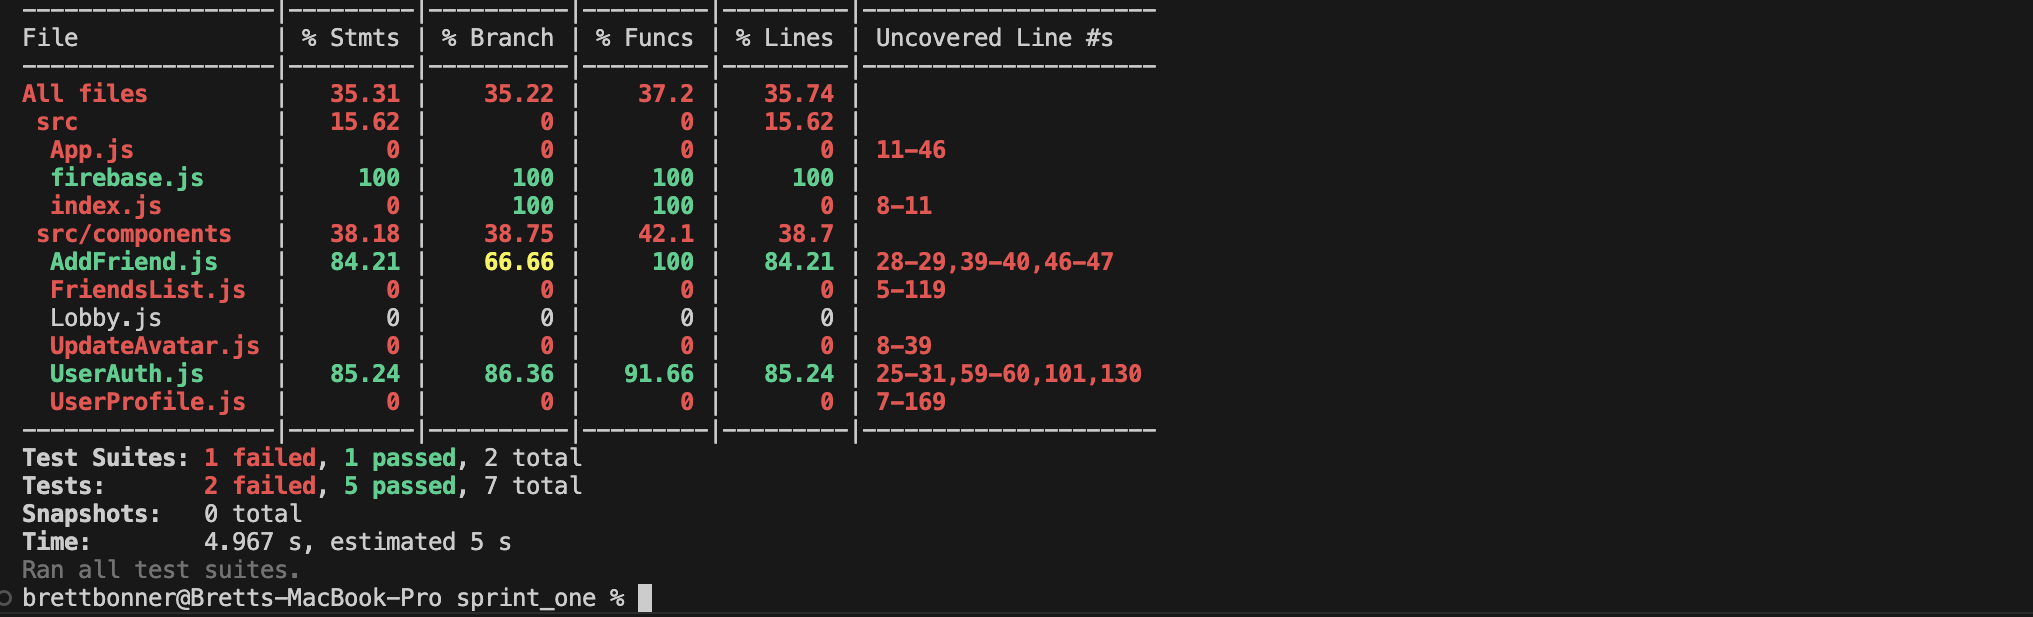
\includegraphics[width=1\linewidth]{figures/Testing-2.png}
    \caption{Sprint 1 Testing Output}
    \label{fig:enter-label}
\end{figure}

    We chose Jest as a testing framework. We attempted to do unit testing for branch and statement coverage, however, we struggled with connecting jest with our react components. We managed to get some of our code tested as shown in firebase.js, AddFriend.js, and UserAuth.js. For our next sprint we plan on solving the issue with testing with a spike to ensure we meet the specified requirements. 


 

\begin{table}[h]
\centering
No story changes or slices during this sprint.

\caption{Sprint 1 Story Distribution and Point Tracking}
\begin{tabular}{|p{3cm}|p{6cm}|c|c|}
\hline
\textbf{Team Member} & \textbf{Stories Attempted} & \textbf{Points Attempted} & \textbf{Status} \\
\hline
Ayoposi Olu & 
\begin{itemize}
    \item S4: Logout (1 pt)
    \item S5: Password (2 pts)
    \item S6: Update (1 pt)
\end{itemize} & 
4 & 
Completed \\
\hline
Jonathan Ramos & 
\begin{itemize}
    \item S7: Profile Avatar (2 pts)
    \item S8: Add Friend (2 pts)
    \item S9: Remove Friend (2 pts)
    \item S10: Show Friends (1 pt)
\end{itemize}& 
7 & 
Completed \\
\hline
Brett Bonner & 
\begin{itemize}
    \item S1: Create User (2 pts)
    \item S2: Guest Account (1 pt)
    \item S3: Login (1 pt)
\end{itemize} & 
4 & 
Completed \\
\hline
\multicolumn{4}{|c|}{} \\
\hline
\multicolumn{2}{|l|}{\textbf{Total Points Attempted}} & \multicolumn{2}{c|}{15} \\
\hline
\multicolumn{2}{|l|}{\textbf{Total Sprint Points (All Stories)}} & \multicolumn{2}{c|}{62} \\
\hline
\end{tabular}

\vspace{0.5cm}
\begin{center}
\small{Sprint 1 period from 10/17/2024 to 10/24/2024}
\end{center}
\end{table}

\begin{table}[h]
\centering
\caption{Team Velocity and Hours-per-Point Metrics}
\begin{tabular}{|l|c|c|c|}
\hline
\textbf{Team Member} & \textbf{Hours Worked} & \textbf{Story Points} & \textbf{Hours/Point} \\
\hline
Ayoposi Olu & 12 & 4 & 3 \\
\hline
Jonathan Ramos & 20 & 7 & 2.85 \\
\hline
Brett Bonner & 13 & 4 & 3.25 \\
\hline
\multicolumn{4}{|c|}{} \\
\hline
\multicolumn{2}{|l|}{\textbf{Team Totals}} & \textbf{14} & \textbf{2.857} \\
\hline
\end{tabular}

\begin{center}
\small{Sprint Velocity History}
\end{center}
\begin{tabular}{|l|c|c|c|c|}
\hline
\textbf{Sprint} & \textbf{Points Completed} & \textbf{Hours Worked} & \textbf{Hours/Point} & \textbf{Velocity} \\
\hline
Sprint 1 & 14 & 45 & 3 & 14 pts/sprint \\
\hline
\end{tabular}

\vspace{0.5cm}
\begin{center}
\small{Velocity = Points completed per sprint \\
Hours/Point = Total hours worked / Points completed}
\end{center}
\end{table}



\subsection{Sprint 2}

\subsubsection{Plan}
User Stories and Technical Tasks attempted in sprint 2 

Brett Bonner
\begin{itemize}
    \item S15: Private Chat (3 pts)
    \item S16: Review Chat (2 pts)
\end{itemize}


Ayoposi Olu

\begin{itemize}
    \item S17: Lobby (5 pts)
    \item Technical Task: Testing (2 pts)
\end{itemize}


Jonathan Ramos

\begin{itemize}
    \item S19: Table (5 pts)
    \item S21: Start Game (3 pts)
    \item S22: Bot (5 pts)
\end{itemize}

\subsubsection{Activities}
During this sprint we built on top of the working deliverable from sprint 1. This sprint began similarly to the last sprint, in which, we set up the database accordingly to handle chats and tables. We added two new collections to our Firestore component, properly names `chats' and `tables'. The chats collection creates a document for every chat that happens between two players. Each chat document has a single field which is an array of maps named messages. Each element in the array is a map containing three fields, senderID, text, and a timestamp. The tables collection creates a document for every table that is created between two players. Each table document has several fields, createdAt, createdBy, maxPlayers, playerIDs (array), players (array), and status. This document is filled appropriately when a player connects to the table. Once the host deals the cards, therefore starting the game, the players array is populated with a deck (array), the currentCard, and the score of each player. This document is essential for the driving the multiplayer game as it is vital that each user obtains the same information from the database in real-time. The tables collection is also necessary to populate our lobby with live tables as user's need to join or create a table to play online. 


\subsubsection{Retrospective}
During this sprint, we planned to complete about the same story points as sprint 1. \textbf{S19 Table}, was a challenging story to complete as it involved writing the entire game logic on the front-end and back-end. Additionally, S19 Table required players to connect and play the game in real-time. During the process of completing this user story, user stories \textbf{S21 Start Game} and \textbf{S22 Bot} were also completed. S22 was completed as the game logic was being developed, it was necessary to play with the computer to ensure the game logic was working properly on both the front-end and back-end. S22 Start Game was completed as when 2 players connected to a table, the host of the game needed to deal the cards and therefore start the game for both players. 

\subsubsection {Testing}
\begin{figure}[h]
    \centering
    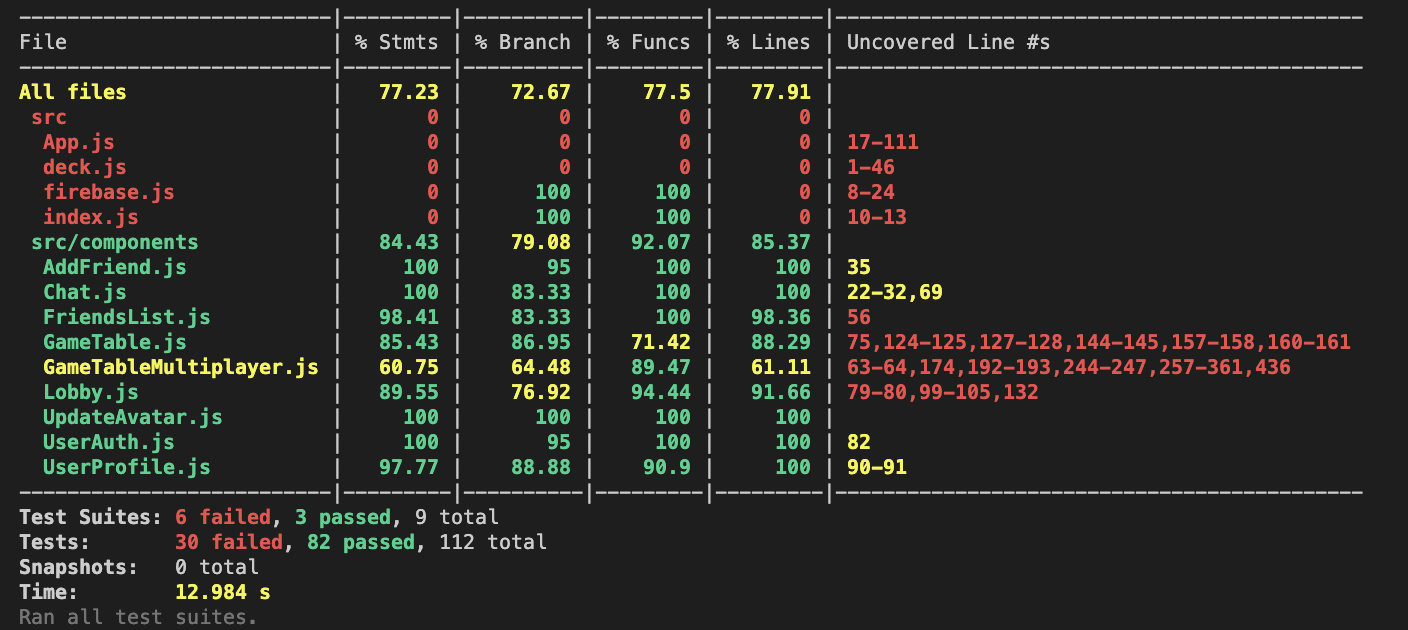
\includegraphics[width=1\linewidth]{figures/Testing.png}
    \caption{Sprint 2 Testing Output}
    \label{fig:enter-label}
\end{figure}

We improved on our testing coverage when compared to our testing coverage from sprint 1. Due to the challenges we faced with our testing framework and its dependencies, we used AI as a tool to help us clean up our testing environment and write tests based on the test cases we provided. We increased our statement coverage for all files to 77.23 percent and increased out branch coverage for all files to 72.67 percent. This is a significant increase when compared to our testing from sprint 1. 
     



\begin{table}[h]
\centering
No story changes or slices during this sprint.

\caption{Sprint 2 Story Distribution and Point Tracking}
\begin{tabular}{|p{3cm}|p{6cm}|c|c|}
\hline
\textbf{Team Member} & \textbf{Stories Attempted} & \textbf{Points Attempted} & \textbf{Status} \\
\hline
Ayoposi Olu & 
\begin{itemize}
    \item S17: Lobby (5 pts)
    \item Technical Task: Testing (2 pts)
\end{itemize} & 
7 & 
Completed \\
\hline
Jonathan Ramos & 
\begin{itemize}
    \item S19: Table (5 pts)
    \item S21: Start Game (3 pts)
    \item S22: Bot (5 pts)
\end{itemize}& 
13 & 
Completed \\
\hline
Brett Bonner & 
\begin{itemize}
    \item S15: Private Chat (3 pts)
    \item S16: Review Chat (2 pts)
\end{itemize} & 
5 & 
Completed \\
\hline
\multicolumn{4}{|c|}{} \\
\hline
\multicolumn{2}{|l|}{\textbf{Total Points Attempted}} & \multicolumn{2}{c|}{25} \\
\hline
\multicolumn{2}{|l|}{\textbf{Total Sprint Points (All Stories)}} & \multicolumn{2}{c|}{62} \\
\hline
\end{tabular}

\vspace{0.5cm}
\begin{center}
\small{Sprint period from 10/24/2024 to 11/07/2024}
\end{center}
\end{table}

\begin{table}[h]
\centering
\caption{Team Velocity and Hours-per-Point Metrics}
\begin{tabular}{|l|c|c|c|}
\hline
\textbf{Team Member} & \textbf{Hours Worked} & \textbf{Story Points} & \textbf{Hours/Point} \\
\hline
Ayoposi Olu & 22 & 7 & 3.14 \\
\hline
Jonathan Ramos & 35 & 13 & 2.69 \\
\hline
Brett Bonner & 15 & 5 & 3.0 \\
\hline
\multicolumn{4}{|c|}{} \\
\hline
\multicolumn{2}{|l|}{\textbf{Team Totals }} & \textbf{25} & \textbf{2.88} \\
\hline
\end{tabular}

\begin{center}
\small{Sprint Velocity History}
\end{center}
\begin{tabular}{|l|c|c|c|c|}
\hline
\textbf{Sprint} & \textbf{Points Completed} & \textbf{Hours Worked} & \textbf{Hours/Point} & \textbf{Velocity} \\
\hline
Sprint 2 & 25 & 72 & 2.88 & 19.5 pts/sprint \\
\hline
\end{tabular}

\vspace{0.5cm}
\begin{center}
\small{Velocity = Points completed per sprint \\
Hours/Point = Total hours worked / Points completed}
\end{center}
\end{table}


\subsection{Sprint 3}

\subsubsection{Plan}
User Stories and Technical Tasks attempted in sprint 3

Brett Bonner
\begin{itemize}
    \item S12: Display Stats (1 pt)
    \item S23: Manage Users (1 pt)
    \item S25: Manage Ads (3 pts)
\end{itemize}


Ayoposi Olu

\begin{itemize}
    \item S27: Notifications (1 pt)
    \item S18: Tutorial (3 pts)
    \item S20: Currency (1 pt)
\end{itemize}


Jonathan Ramos

\begin{itemize}
    \item S19: Table (5 pts)
    \item S21: Start Game (3 pts)
    \item S22: Bot (5 pts)
\end{itemize}

\subsubsection{Activities}
During this sprint we focused on completing admin user stories as we had not completed any admin functionalities yet. S19 Table was placed on the backlog for additional work. During this sprint, the user interface for the game was updated to become more interactive for the user. Additionally, we improved the logic for War to handle back-to-back wars when playing with a bot. As for multiplayer, we improved the user interface to becomes more interactive for both players. During this sprint we encountered an issue with the multiplayer game in which the system would read from the database a significant amount more than it needed to. Due to the high number of reads, we reached the limits of our database and unfortunately lost time in waiting for our quota to clear. This issue was fixed during this sprint, the multiplayer component was updated to only read from the database when the status field is updated, this greatly reduced the number of reads, and therefore fixing the issue. However, due to this unforeseen event, the tie-breaker (war) for multiplayer does not follow the traditional rules of the game. Due to time constraints, our multiplayer game handles war by returning each card back to the player that placed it. Display Stats and Manage Ads were both attempted and completed, however Manage users was not completed during this sprint. 


\subsubsection{Retrospective}
\textbf{S19 Table}, remained a challenging story to complete. Due to the unforeseen obstacle we faced with our database, we lost several hours of time needed to work on fully completing all of the features of the game. We also ran into issues with testing \textbf{S22 Bot} as the game logic changed from sprint 2 to support back-to-back wars. The user interface was also significantly changed from sprint 2. These changes caused our previous tests to no longer work as they depended on the structure of our previous code. Similarly, \textbf{S19 Table} was also significantly changed from sprint 2 to sprint 3 to support a more interactive user interface as well as updating the game logic to support the updated interactivity. The development of a tutorial was necessary during this sprint as we needed a way to give users a smooth understanding of the card game. Additionally, a simple currency was implemented into the game to add stakes for each a table. Notifications were implemented during this sprint as a functionality for an admin user, in which only they can send and modify notifications that go out to all users. One of the ways we could have been more efficient was to complete the multiplayer game first and build the supporting features around it. The multiplayer part quickly became more difficult than it seemed at first which resulted in time lost waiting for the table component to be completed. 


\subsubsection {Testing}
\begin{figure}[h]
    \centering
    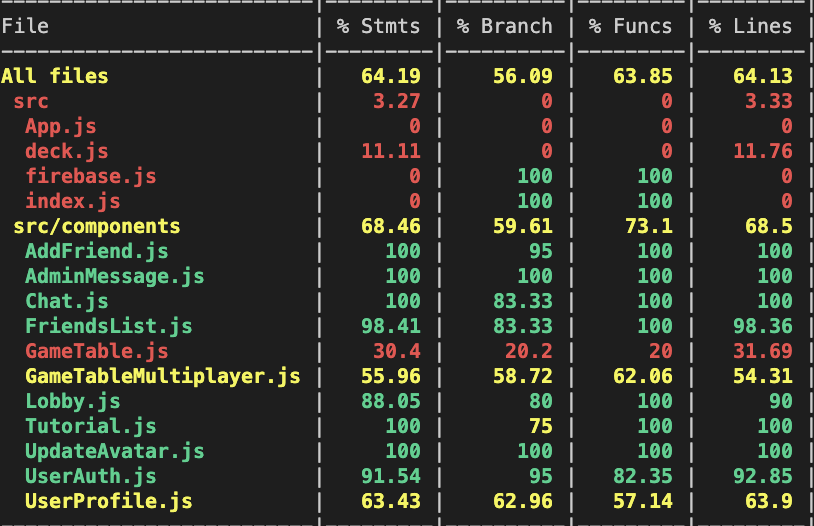
\includegraphics[width=1\linewidth]{documentation/figures/Testing sprint 3.png}
    \caption{Sprint 2 Testing Output}
    \label{fig:enter-label}
\end{figure}
Testing unfortunately decreased during this sprint due to the significant changes made to GameTable.js and GameTableMultiplayer.js. We also created tests for AdminMessage.js and Tutorial.js which were created during this sprint. 

     



\begin{table}[h]
\centering
No story changes or slices during this sprint.

\caption{Sprint 3 Story Distribution and Point Tracking}
\begin{tabular}{|p{3cm}|p{6cm}|c|c|}
\hline
\textbf{Team Member} & \textbf{Stories Attempted} & \textbf{Points Attempted} & \textbf{Status} \\
\hline
Ayoposi Olu & 
\begin{itemize}
    \item S27: Notifications (1 pt)
    \item S18: Tutorial (3 pts)
    \item S20: Currency (1 pt)
\end{itemize} & 
5 & 
Completed \\
\hline
Jonathan Ramos & 
\begin{itemize}
    \item S19: Table (5 pts)
    \item S21: Start Game (3 pts)
    \item S22: Bot (5 pts)
\end{itemize}& 
13 & 
Completed \\
\hline
Brett Bonner & 
\begin{itemize}
    \item S12: Display Stats (1 pt)
    \item S23: Manage Users (1 pt)
    \item S25: Manage Ads (3 pts)
\end{itemize} & 
5 & 
Completed \\
\hline
\multicolumn{4}{|c|}{} \\
\hline
\multicolumn{2}{|l|}{\textbf{Total Points Attempted}} & \multicolumn{2}{c|}{23} \\
\hline
\multicolumn{2}{|l|}{\textbf{Total Sprint Points (All Stories)}} & \multicolumn{2}{c|}{62} \\
\hline
\end{tabular}

\vspace{0.5cm}
\begin{center}
\small{Sprint period from 11/07/2024 to 11/21/2024}
\end{center}
\end{table}

\begin{table}[h]
\centering
\caption{Team Velocity and Hours-per-Point Metrics}
\begin{tabular}{|l|c|c|c|}
\hline
\textbf{Team Member} & \textbf{Hours Worked} & \textbf{Story Points} & \textbf{Hours/Point} \\
\hline
Ayoposi Olu & 16 & 5 & 3.2 \\
\hline
Jonathan Ramos & 25 & 13 & 1.92 \\
\hline
Brett Bonner & 13 & 5 & 2.6 \\
\hline
\multicolumn{4}{|c|}{} \\
\hline
\multicolumn{2}{|l|}{\textbf{Team Totals }} & \textbf{23} & \textbf{2.34} \\
\hline
\end{tabular}

\begin{center}
\small{Sprint Velocity History}
\end{center}
\begin{tabular}{|l|c|c|c|c|}
\hline
\textbf{Sprint} & \textbf{Points Completed} & \textbf{Hours Worked} & \textbf{Hours/Point} & \textbf{Velocity} \\
\hline
Sprint 1 & 14 & 45 & 3 & 14 pts/sprint \\
\hline
Sprint 2 & 25 & 72 & 2.88 & 19.5 pts/sprint \\
\hline
Sprint 3 & 23 & 54 & 2.34 & 20.33 pts/sprint \\
\hline
\end{tabular}

\vspace{0.5cm}
\begin{center}
\small{Velocity = Points completed per sprint \\
Hours/Point = Total hours worked / Points completed}
\end{center}
\end{table}
